\documentclass[12pt, letterpaper]{article}
\usepackage[a4paper, margin=1in]{geometry}
\usepackage{amsmath}
\usepackage{graphicx}
\usepackage{float}
\graphicspath{{images/}}
\author{Joseph Yu}
\title{Lab 4: Neural Coding}
\begin{document}
\maketitle
\setcounter{section}{3}
\subsection{Grid Score and Manifold Distance}
The Grid Score for a grid cell's rate map is a measure of its hexagonal and square symmetry by rotating the rate map $60\deg$ or $120\deg$ for hexagonal and $90\deg$ for square symmetry and then measuring the correlation between rotated and original. A grid cell's rate map is generated for each grid cell by plotting its activation based on each location within a $res\ x\ res$ grid. When calculating the manifold distance between rate maps we are trying to understand the similarity in activations between the grid cells with the highest grid scores. The similarity can be measured by first picking an origin point within our $res\ x\ res$ grid and then calculating the distance between the top grid cell activations for that origin point and the top grid cell activations for all other points. Below we show the empirical demonstration of the Grid Score and Manifold Distance for learned grid cells in a artificial neural network.

\subsubsection{Grid Score}

Below we break down the grid cells into groups of high, medium, and low grid scores specifically for the hexagonal symmetry. 

\begin{figure}[H]
    \centering
    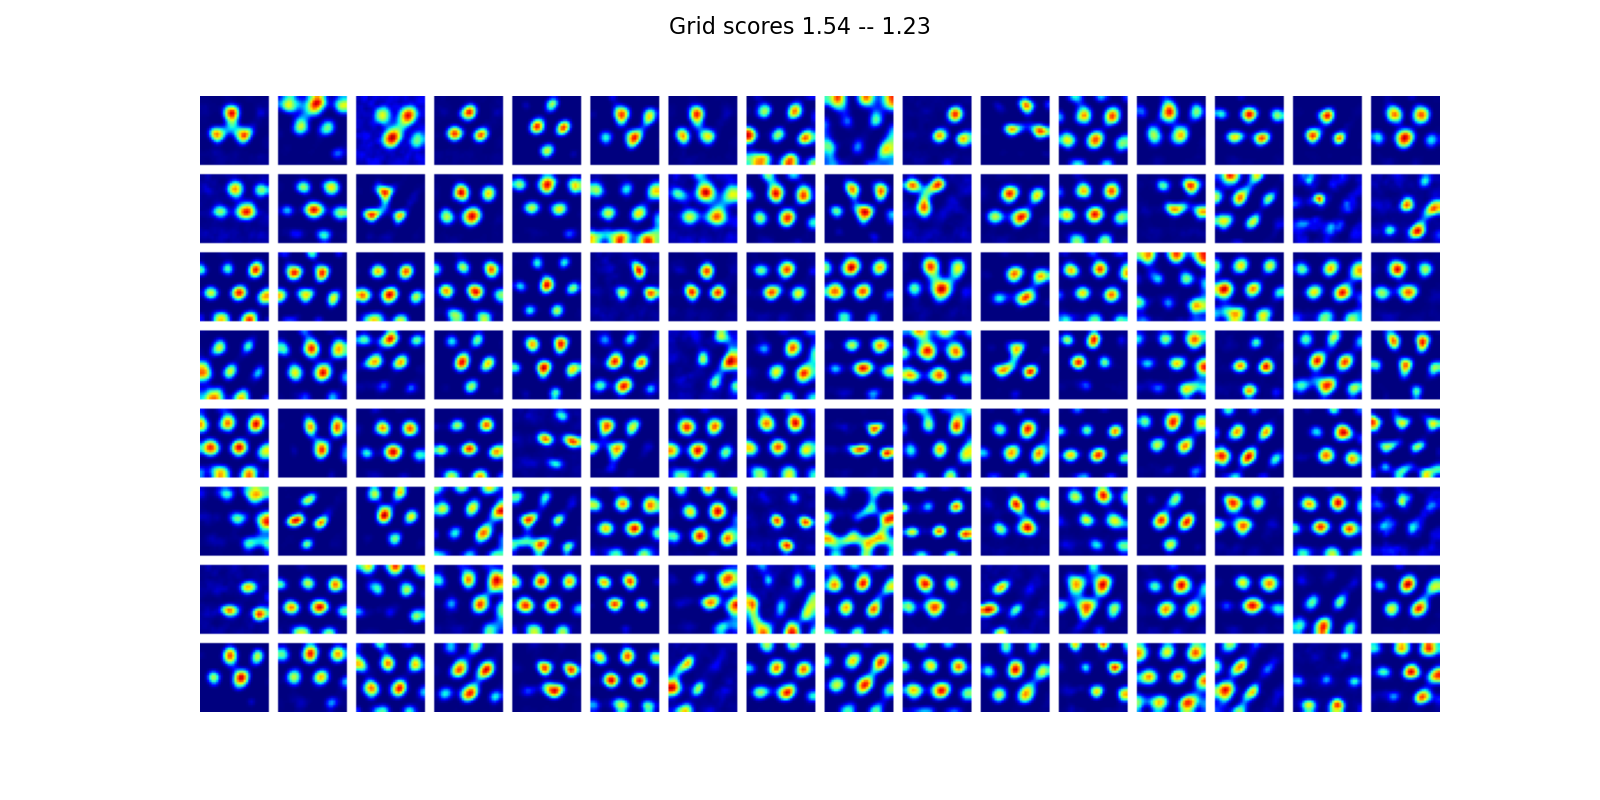
\includegraphics[width=0.8\textwidth]{high_grid_scores.png}
    \caption{High Grid Score for Hexagonal Symmetry}
    \label{fig:high_grid_scores}
\end{figure}

We can see that the grid cells with high grid scores for hexagonal symmetry have a clear hexagonal pattern in their rate maps. This aligns with our understanding of how the grid scores are calculated and what they represent.

\begin{figure}[H]
    \centering
    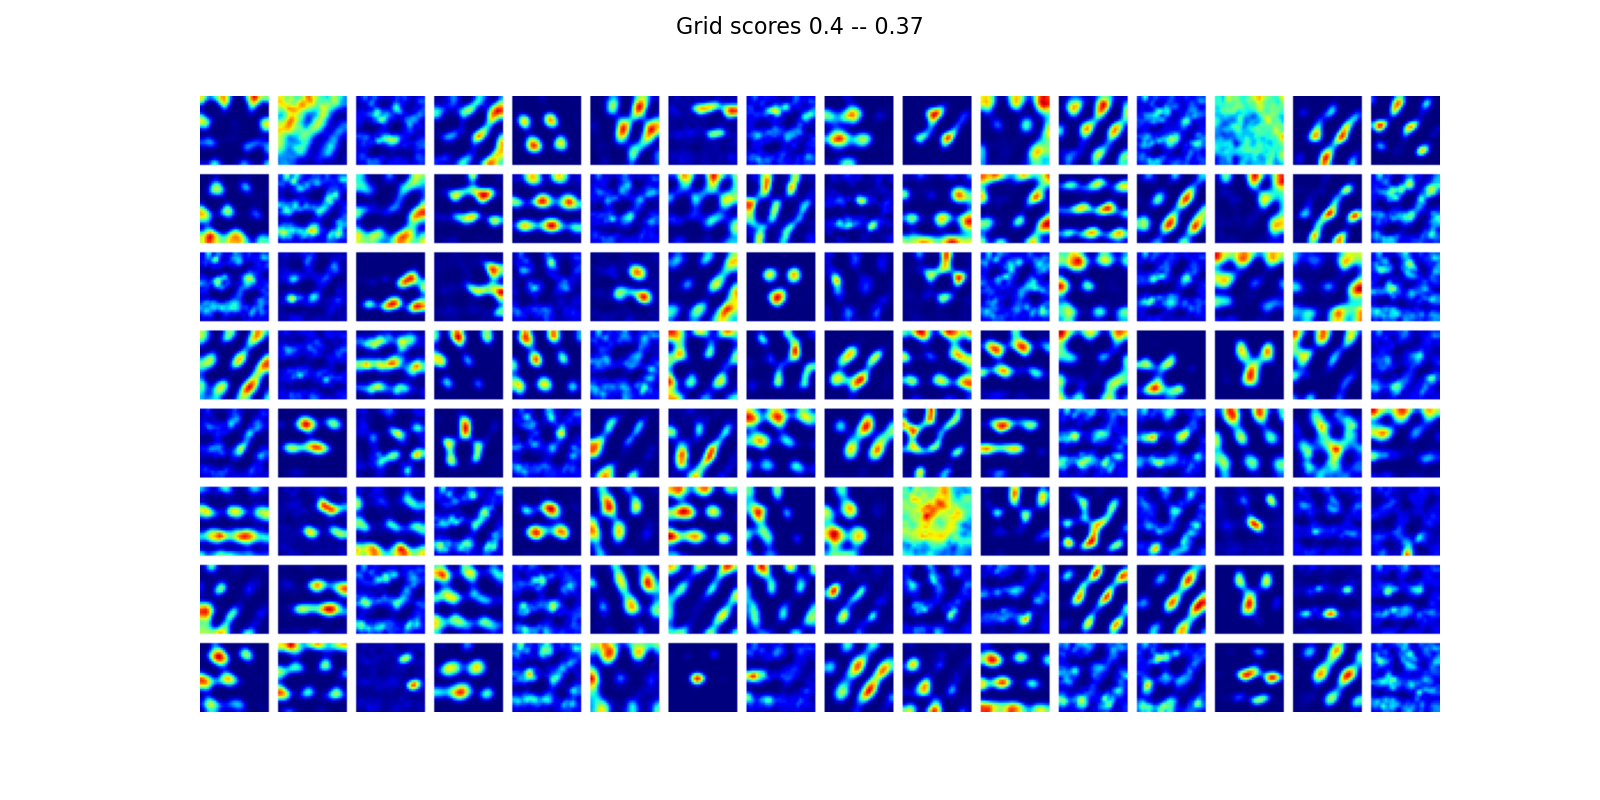
\includegraphics[width=0.8\textwidth]{medium_grid_scores.png}
    \caption{Medium Grid Score for Hexagonal Symmetry}
    \label{fig:medium_grid_scores}
\end{figure}

The grid cells with medium grid scores for hexagonal symmetry have a less clear hexagonal pattern in their rate maps compared to the grid cells with high grid scores. The rate maps for these grid cells are more noisy and less structured.

\begin{figure}[H]
    \centering
    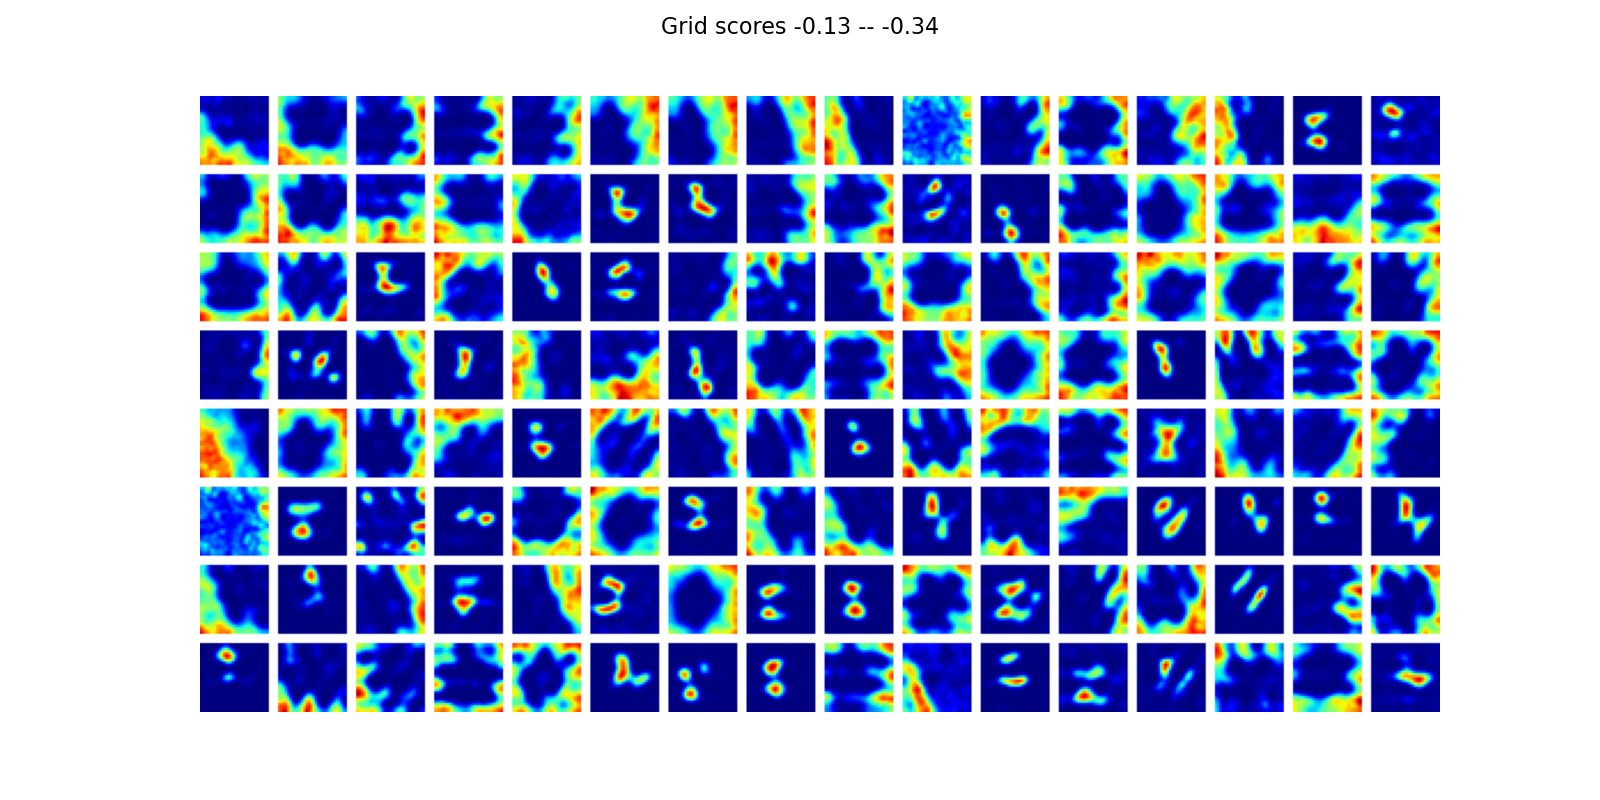
\includegraphics[width=0.8\textwidth]{low_grid_scores.png}
    \caption{Low Grid Score for Hexagonal Symmetry}
    \label{fig:low_grid_scores}
\end{figure}

The grid cells with low grid scores for hexagonal symmetry have no clear hexagonal pattern in their rate maps. The rate maps for these grid cells are very noisy and while some do show structural patterns they are not hexagonal leading to their negative grid scores.

Finally we can also visualize the overall distribution of grid scores across all grid cells.

\begin{figure}[H]
    \centering
    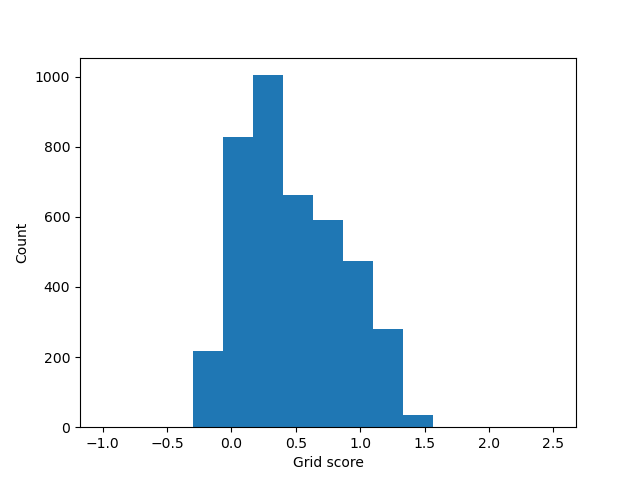
\includegraphics[width=0.8\textwidth]{grid_score_histogram.png}
    \caption{Distribution of Grid Scores for Hexagonal Symmetry}
    \label{fig:grid_score_histogram}
\end{figure}

We can see from the distribution that a majority of the grid scores are positive which indicates that the rate maps for the grid cells have some hexagonal pattern but not a strong hexagonal structure since we don't see a large number of grid scores above 1.


\subsubsection{Manifold Distance}

When calculating the manifold distance we pick $9$ different origin points within our $res\ x\ res$ grid and calculate the Euclidian distance between the top grid cell activations for each origin point and the top grid cell activations for all other points. We can expect to see that for at least the origin point there should be $0$ manifold distance but we should also see a hexagonal structure in the manifold distance plot. The main explanation is that for the top grid score activations it should be repeated in a hexagonal shape across the grid so the origin points activations should not be unique and should also follow this structure. Below we show the empirical demonstration of the manifold distance for learned grid cells in an artificial neural network.

\begin{figure}[H]
    \centering
    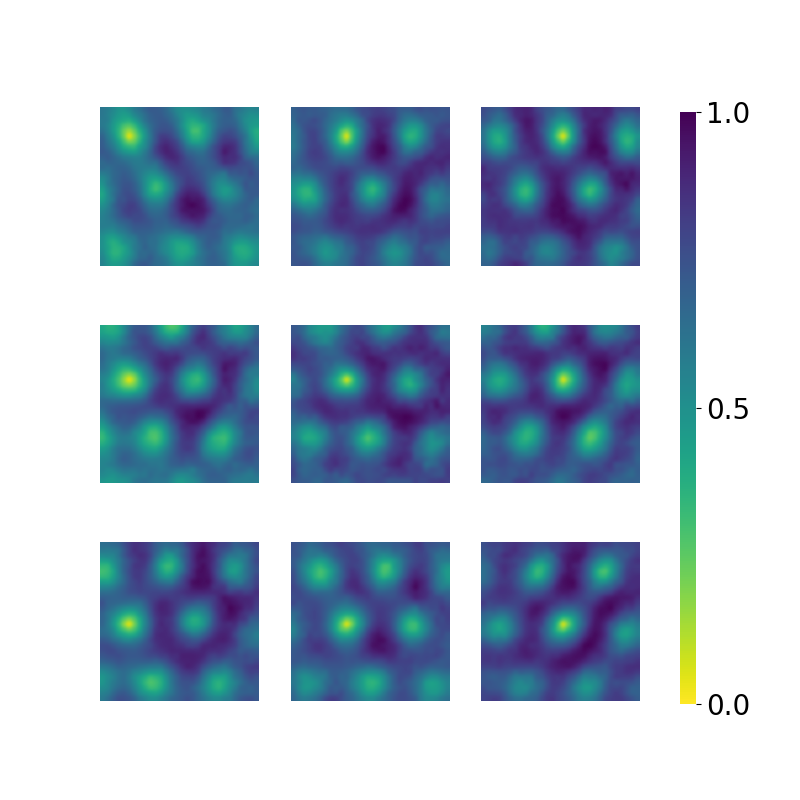
\includegraphics[width=0.8\textwidth]{rate_map_manifold_distance.png}
    \caption{Manifold Distance for Rate Maps of Grid Cells Using $9$ Different Origin Points}
    \label{fig:rate_map_manifold_distance}
\end{figure}

In the figure above the darker regions are high manifold distance meaning less similarity in activations and the brighter areas are low manifold distances. We can clearly see from the figure where the origin points are within the grid since they are the brightest points that have a manifold distance of $0$. However, we can also notice that there is a hexagonal structure in the manifold distances with bright points throughout the grid. This demonstrates that the activations for a single origin point is not unique across the grid. 



\subsection{Neuron coding strategy: population coding and Bayesian decoder}

We want to explore population coding from a Bayesian perspective. In population coding, neurons will have a preferred stimulus i.e. orientation and we can measure a neuron's responses to a wide variety of stimulus to roughly create a distribution of responses. For the Bayesian decoder we want to estimate a posterior distribution for $P(s|r)$ or the probability of a stimulus given a response. From bayes rule 
\[ P(s|r) = \frac{P(r|s)P(s)}{P(r)} \] where $P(r|s)$ is the likelihood of a response given a stimulus, $P(s)$ is the prior probability of a stimulus, and $P(r)$ is the marginal probability of a response. We can describe the likelihood $P(r|s)$ as being equal to the multiplication of $N$ independent Gaussians where $N$ is the number of neurons. Lets say for neuron $i$ $P(r_i|s)$ is Gaussian with mean $\mu_{s}^i$ and a variance of $1$ and the value of $\mu_{s}^i$ is neuron $i$'s expected response when given a stimulus $s$. Then we can calculate the likelihood $P(r|s)$ as
\[ P(r|s) = \prod_{i=1}^{N} P(r_i|s) = \prod_{i=1}^{N} \frac{1}{\sqrt{2\pi}}e^{-\frac{1}{2}(r_i - \mu_{s}^i)^2} = \frac{1}{{\sqrt{2\pi}}^N}e^{-\frac{1}{2}\sum_{i=1}^{N}(r_i - \mu_{s}^i)^2}\]

To find $\mu_{s}^i$ we can leverage each neuron's tuning curve and then take the density value of the tuning curve at $s$. In this case we also assume that each neuron's tuning curve is a Gaussian distribution with $\mu$ equal to the neuron's preferred stimulus. The prior $P(s)$ is the uniform distribution since we don't have any prior knowledge of any stimulus being more likely. The marginal probability $P(r)$ is the sum of the likelihoods for all possible stimuli. We can then use the likelihood, prior, and marginal probability to calculate the posterior $P(s|r)$ which will give us the probability of a stimulus given a response. Below we show the empirical demonstration of the Bayesian decoder for population coding.

First lets take a look at an example of a neuron's tuning curve. We will use three neurons as an example each with different preferred stimulus orientations.

\begin{figure}[H]
    \centering
    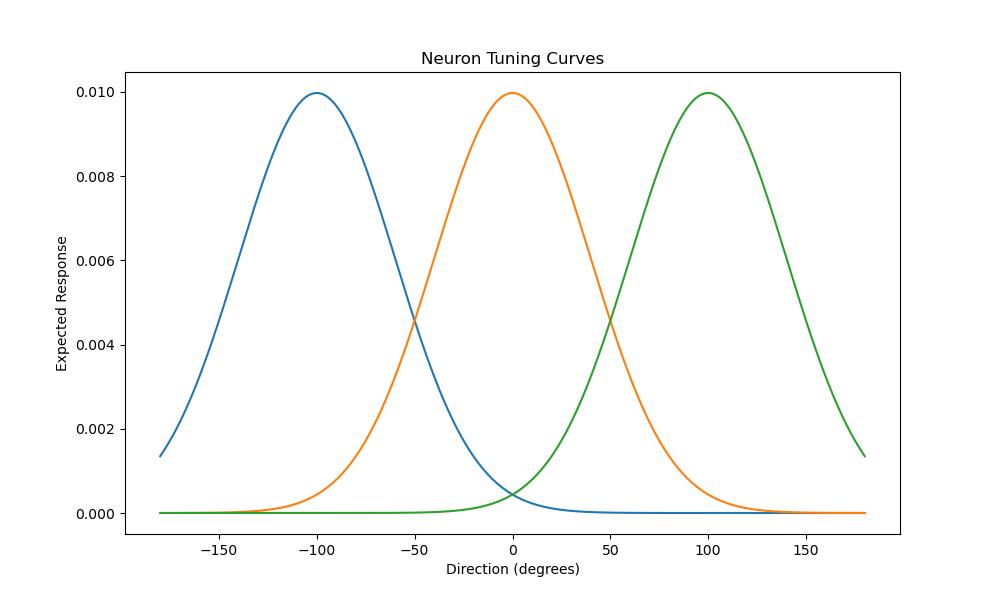
\includegraphics[width=0.8\textwidth]{3_neuron_tuning_curves.png}
    \caption{Tuning Curves for Three Neurons with Different Preferred Stimulus Orientations}
    \label{fig:3_neuron_tuning_curves}
\end{figure}

We can see that each neuron has a Gaussian tuning curve with the largest density or expected response at their preferred stimulus orientation.

Next lets plot the posterior distribution for the Bayesian decoder for population coding. For the following example we have a set true stimulus orientation and a set of responses from $50$ neurons. We can then calculate the posterior distribution for the true stimulus orientation given the responses from the neurons.

\begin{figure}[H]
    \centering
    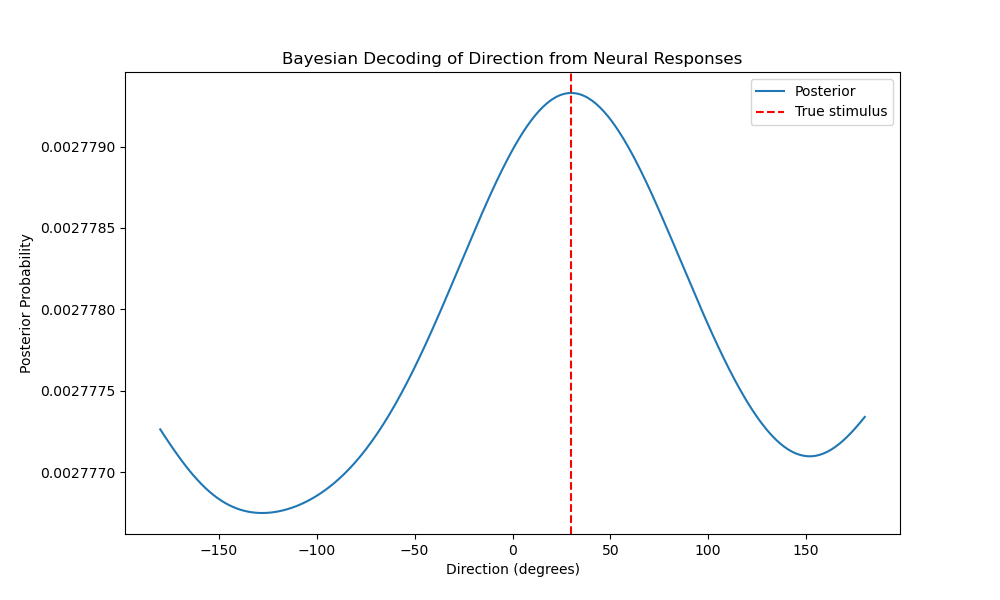
\includegraphics[width=0.8\textwidth]{bayesian_decoder.png}
    \caption{Posterior Distribution for Bayesian Decoder for Population Coding}
    \label{fig:bayesian_decoder}
\end{figure}

We can see that the posterior distribution for the Bayesian decoder is centered around the true stimulus orientation which has the highest density value. We can also notice that the posterior is not a Gaussian distribution but potentially one that is actually multi-modal since the density seems to increase near the $-180$ and $180$ stimulus orientations. 

\subsection{FlyLSH}
Here we explore an alternative to the standard LSH algorithm called FlyLSH. The goal of LSH algorithms is to using a random projection matrix to introduce a hashed version of the input. Similar inputs we expect to see similar hashes which means we can use a nearest neighbors algorithm to make predictions on the class of the input. FlyLSH is a variant of LSH that is biologically inspired by the fly brain and its olfactory system. It uses a random sparse binary projection matrix rather than the traditional dense Gaussian projection matrix. Another difference is that FlyLSH increases dimensionality while LSH will reduce dimensionality. Finally, FlyLSH leverages a winner-take-all mechanism to select the top $k$ hash codes for a given input. Below we show the empirical demonstration of FlyLSH on the MNIST dataset.

First we can take a look at how FlyLSH performs on accuracy and hash calculation duration for a variety of output dimension values. 

\begin{figure}[H]
    \centering
    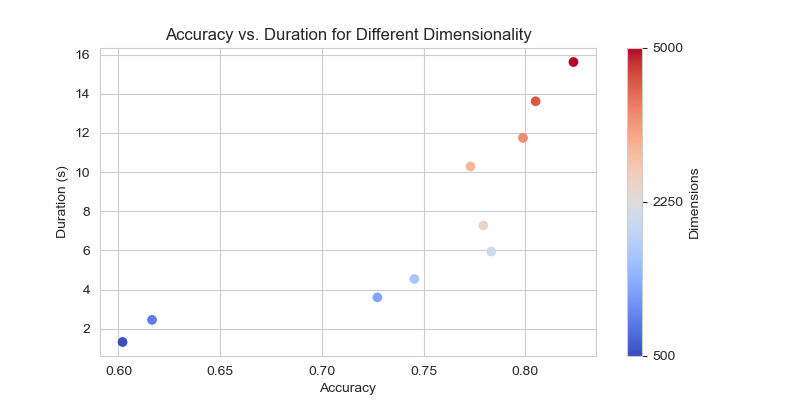
\includegraphics[width=0.8\textwidth]{fly_hash.png}
    \caption{Accuracy of FlyLSH on MNIST Dataset for Different Output Dimensions}
    \label{fig:fly_hash}
\end{figure}

The figure above plots the accuracy of FlyLSH on the MNIST dataset on the x-axis and the duration on the y-axis. It is also colored based on the output dimension size. We can see that as the output dimension size increases the accuracy of FlyLSH also increases and so does the hash calculation duration. This is expected since increasing the output dimension size will increase the number of hash codes that can be generated and thus increase the accuracy of the algorithm. However, this will also increase the time it takes to calculate the hash codes. We can further plot the output dimension size against the accuracy and hash calculation duration to see how they are related.

\begin{figure}[H]
    \centering
    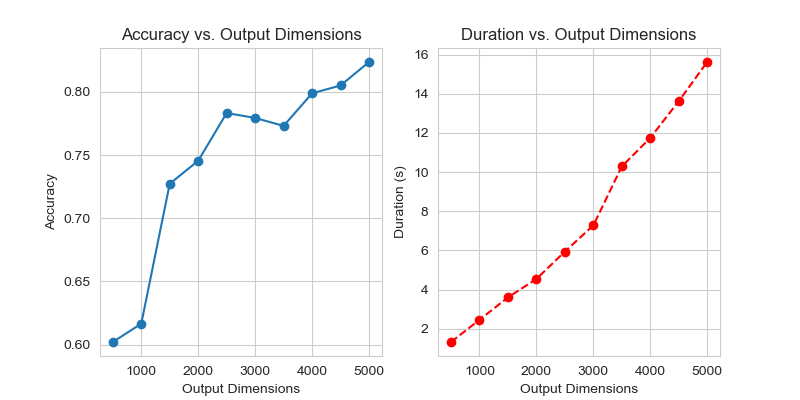
\includegraphics[width=0.8\textwidth]{fly_hash_compare_dim_accuracy_duration.png}
    \caption{Accuracy and Hash Calculation Duration of FlyLSH on MNIST Dataset for Different Output Dimensions}
    \label{fig:fly_hash_compare_dim_accuracy_duration}
\end{figure}

As the output dimension size increases the accuracy of FlyLSH also increases. However, for smaller output dimensions the accuracy increases at a much faster rate than for larger output dimensions demonstrating that there is a logarithmic relationship between the output dimension size and the accuracy. The hash calculation duration also increases as the output dimension size increases but for larger output dimensions the increase in duration is much more significant. This suggests that there is an exponential relationship between the output dimension size and the hash calculation duration.

To compare the performance of FlyLSH with LSH we can plot the accuracy based on the hash length for both algorithms. The hash length is the number of non-zero elements in the final hash code. For normal LSH we saw a $92\%$ accuracy with a hash length of $128$.

\begin{figure}[H]
    \centering
    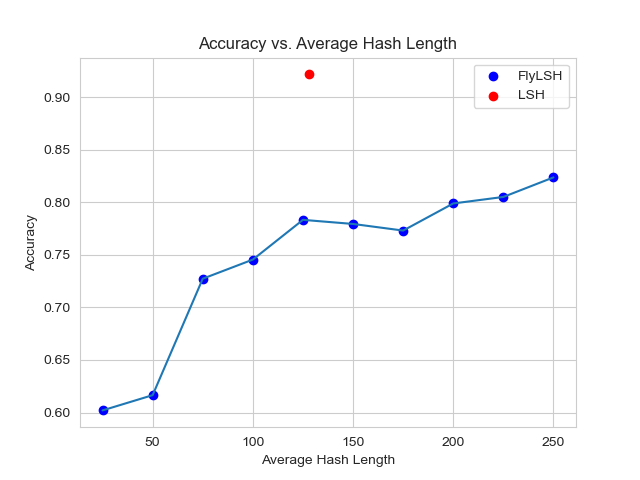
\includegraphics[width=0.8\textwidth]{fly_hash_compare_hash_length.png}
    \caption{Accuracy of FlyLSH and LSH on MNIST Dataset for Different Hash Lengths}
    \label{fig:fly_hash_compare_hash_length}
\end{figure}

The red point denotes the accuracy of LSH with a hash length of $128$ and the blue points denote the accuracy of FlyLSH for different output dimensions. We can see that for the same hash length FlyLSH is significantly less accurate than LSH. Even at double the hash length of LSH, FlyLSH is still less accurate. 

\subsection{Head Direction Tuning Curves}
For each grid cell we can visualize its head direction tuning curve or its activation based on a specific heading direction. In order to do this we break down the the possible heading directions between $-\pi$ and $\pi$ into $10$ bins and then calculate the average activation for each bin. The following figure shows $100$ head direction tuning curves for $100$ grid cells. The specific ordering of the tuning curves is actually based on the first and second principal components of the tuning curves. With the top left corner being the grid cell with the lowest first principal component and the lowest second principal component and the bottom right corner being the grid cell with the highest first principal component and the highest second principal component. The first principal component values increase across the x-axis and the second principal component values increase across the y-axis.

\begin{figure}[H]
    \centering
    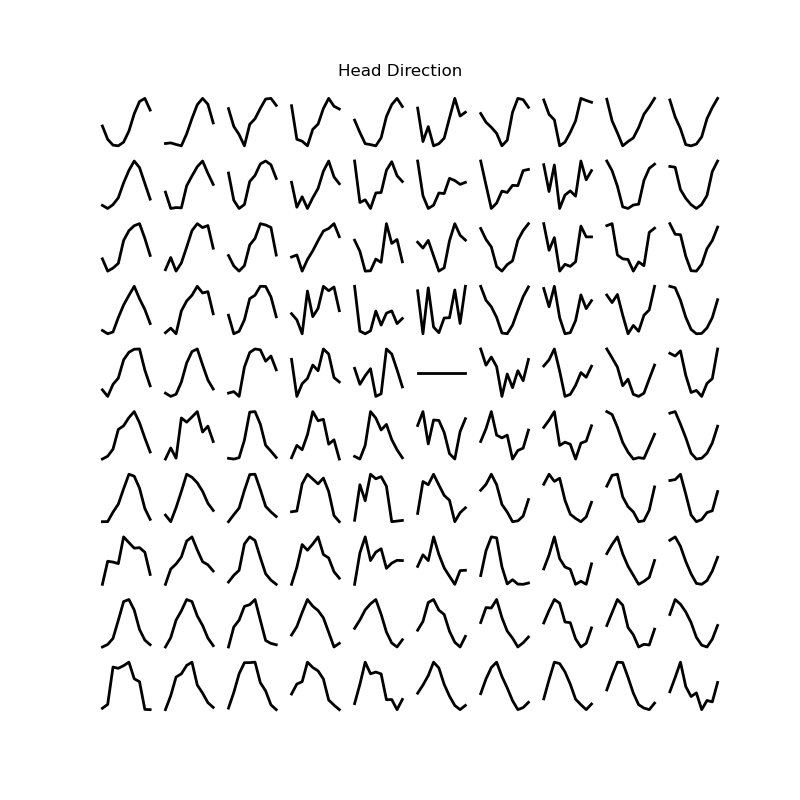
\includegraphics[width=0.8\textwidth]{head_direction.png}
    \caption{Head Direction Tuning Curves for $100$ Grid Cells}
    \label{fig:head_direction}
\end{figure}

We can notice from the figure that for large first principal component values the head direction tuning curves show higher activations at the extremes of the heading directions while for large second principal component values the head direction tuning curves show higher activations at the center of the heading directions. Moving along the x-axis and y-axis we can visualize the flipping of the tuning curves peak activations. In the middle of the figure theres also a tuning curve with no activations which means that some grid cells are not tuned to any specific heading direction and those flat tuning curves have a first and second principal component value roughly in the middle of the range.
\end{document}